\hypertarget{CImg_8display_8cpp}{
\section{CImg.display.cpp File Reference}
\label{CImg_8display_8cpp}\index{CImg.display.cpp@{CImg.display.cpp}}
}
{\tt \#include \char`\"{}CImg.h\char`\"{}}\par
{\tt \#include $<$iostream$>$}\par


Include dependency graph for CImg.display.cpp:\nopagebreak
\begin{figure}[H]
\begin{center}
\leavevmode
\includegraphics[width=82pt]{CImg_8display_8cpp__incl}
\end{center}
\end{figure}
\subsection*{Defines}
\begin{CompactItemize}
\item 
\#define \hyperlink{CImg_8display_8cpp_ea1ac050c1347d4a67f85cbfc88ec8cf}{PR}(value)~;
\end{CompactItemize}
\subsection*{Functions}
\begin{CompactItemize}
\item 
{\footnotesize template$<$typename T$>$ }\\void \hyperlink{CImg_8display_8cpp_1ddf6ad29b94342df84bf770d6d90b11}{display1D2D} (CImg$<$ T $>$ image)
\begin{CompactList}\small\item\em display image as both 2D map and 1D graphs along x or y axis \item\end{CompactList}\item 
{\footnotesize template$<$typename T$>$ }\\void \hyperlink{CImg_8display_8cpp_b599c0258589192cac899b35ef432ce0}{display3D} (CImg$<$ T $>$ image, const char $\ast$file\_\-o, const float ratioz, const unsigned int di, const char $\ast$file\_\-pose\_\-i, const char $\ast$file\_\-pose\_\-o, unsigned int rtype, bool color\_\-type)
\begin{CompactList}\small\item\em display image as 3D surface \item\end{CompactList}\item 
int \hyperlink{CImg_8display_8cpp_3c04138a5bfe5d72780bb7e82a18e627}{main} (int argc, char $\ast$$\ast$argv)
\end{CompactItemize}


\subsection{Define Documentation}
\hypertarget{CImg_8display_8cpp_ea1ac050c1347d4a67f85cbfc88ec8cf}{
\index{CImg.display.cpp@{CImg.display.cpp}!PR@{PR}}
\index{PR@{PR}!CImg.display.cpp@{CImg.display.cpp}}
\subsubsection[PR]{\setlength{\rightskip}{0pt plus 5cm}\#define PR(value)~;}}
\label{CImg_8display_8cpp_ea1ac050c1347d4a67f85cbfc88ec8cf}




Definition at line 168 of file CImg.display.cpp.

\subsection{Function Documentation}
\hypertarget{CImg_8display_8cpp_1ddf6ad29b94342df84bf770d6d90b11}{
\index{CImg.display.cpp@{CImg.display.cpp}!display1D2D@{display1D2D}}
\index{display1D2D@{display1D2D}!CImg.display.cpp@{CImg.display.cpp}}
\subsubsection[display1D2D]{\setlength{\rightskip}{0pt plus 5cm}template$<$typename T$>$ void display1D2D (CImg$<$ T $>$ {\em image})\hspace{0.3cm}{\tt  \mbox{[}inline\mbox{]}}}}
\label{CImg_8display_8cpp_1ddf6ad29b94342df84bf770d6d90b11}


display image as both 2D map and 1D graphs along x or y axis 

\begin{Desc}
\item[Parameters:]
\begin{description}
\item[\mbox{$\leftarrow$} {\em image}]: image to display \end{description}
\end{Desc}


Definition at line 176 of file CImg.display.cpp.

Here is the caller graph for this function:\nopagebreak
\begin{figure}[H]
\begin{center}
\leavevmode
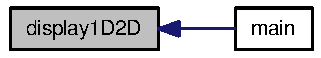
\includegraphics[width=95pt]{CImg_8display_8cpp_1ddf6ad29b94342df84bf770d6d90b11_icgraph}
\end{center}
\end{figure}
\hypertarget{CImg_8display_8cpp_b599c0258589192cac899b35ef432ce0}{
\index{CImg.display.cpp@{CImg.display.cpp}!display3D@{display3D}}
\index{display3D@{display3D}!CImg.display.cpp@{CImg.display.cpp}}
\subsubsection[display3D]{\setlength{\rightskip}{0pt plus 5cm}template$<$typename T$>$ void display3D (CImg$<$ T $>$ {\em image}, \/  const char $\ast$ {\em file\_\-o}, \/  const float {\em ratioz}, \/  const unsigned int {\em di}, \/  const char $\ast$ {\em file\_\-pose\_\-i}, \/  const char $\ast$ {\em file\_\-pose\_\-o}, \/  unsigned int {\em rtype}, \/  bool {\em color\_\-type})\hspace{0.3cm}{\tt  \mbox{[}inline\mbox{]}}}}
\label{CImg_8display_8cpp_b599c0258589192cac899b35ef432ce0}


display image as 3D surface 

\begin{Desc}
\item[Parameters:]
\begin{description}
\item[\mbox{$\leftarrow$} {\em image}]: image to display \end{description}
\end{Desc}


Definition at line 330 of file CImg.display.cpp.

Here is the caller graph for this function:\nopagebreak
\begin{figure}[H]
\begin{center}
\leavevmode
\includegraphics[width=89pt]{CImg_8display_8cpp_b599c0258589192cac899b35ef432ce0_icgraph}
\end{center}
\end{figure}
\hypertarget{CImg_8display_8cpp_3c04138a5bfe5d72780bb7e82a18e627}{
\index{CImg.display.cpp@{CImg.display.cpp}!main@{main}}
\index{main@{main}!CImg.display.cpp@{CImg.display.cpp}}
\subsubsection[main]{\setlength{\rightskip}{0pt plus 5cm}int main (int {\em argc}, \/  char $\ast$$\ast$ {\em argv})}}
\label{CImg_8display_8cpp_3c04138a5bfe5d72780bb7e82a18e627}




\begin{Desc}
\item[\hyperlink{todo__todo000003}{Todo}]add doxygen comments for main, within the main and \hyperlink{CImg_8display_8cpp_ea1ac050c1347d4a67f85cbfc88ec8cf}{PR()} \end{Desc}


pre-processing

display as image (2D map) and profiles (1D graph)

display as surface (3D)

display as 2D map 

Definition at line 457 of file CImg.display.cpp.

Here is the call graph for this function:\nopagebreak
\begin{figure}[H]
\begin{center}
\leavevmode
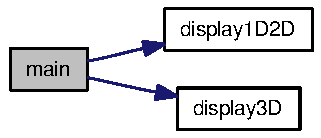
\includegraphics[width=95pt]{CImg_8display_8cpp_3c04138a5bfe5d72780bb7e82a18e627_cgraph}
\end{center}
\end{figure}
